\begin{figure}[htb]
\begin{center}
  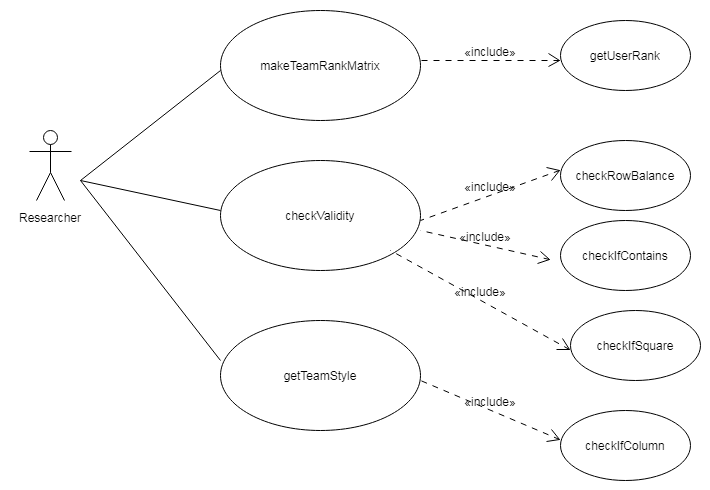
\includegraphics[width=\textwidth,keepaspectratio=true]{rank_functionalRequirements}
\end{center}
\caption{Services to determine the participatory style of a user based on ranking \label{fig:rank_functionalRequirements}}
\end{figure}

Figure \ref{fig:rank_functionalRequirements} shows the lower level services required to determine the participatory style of a user based on ranking. The services are the following:

\begin{description}

\item[makeTeamRankMatrix] The service takes the teamID as parameter and create a rank object for the team. The object is a square matrix with the number columns and the number of rows the same as the number of members in the team. The values entered in each row are determined using the \texttt{getUserRank} service described below for each of the users. 



\item[checkValidity] The services uses \texttt{checkIfContains}, \texttt{checkRowBalance} and \texttt{checkIfSquare} to check the validity of the matrix.



\item[getTeamStyle] This service takes a matrix as a parameter and returns a list of participatory style for each team. It uses \texttt{checkIfColumn} service describes below for each of the users.



 


\end{description}  
The following are helper functions that should be implemented to provide the above services:
\begin{description}
	
	\item[checkIfContains] The service takes the matrix as a parameter and checks if it contains 0,1,3 only and returns a bool.
	
	\item[checkIfSquare] The service takes a matrix as a paremeter and checks if the matrix is a square matrix.
	
	\item[checkIfColumn] The service takes a matrix as a parameter and checks if each column of the matrix and it return a high string and low list.
	
	\item[CheckRowBalance] The service takes a matrix as a parameter and checks each row has the correct composition.
	
	\item[getUserRank] The service takes the teamID and userID as parameter and returns a vector of integer values representing the rankings of the members of the team as reported by the user. 
	
	
	
\end{description}









